%!TEX root = "../../../DA_GUI.tex"

%	--------------------------------------------------------
% 		Wissenschaftliche Analyse: Benutzeroberfläche
%	--------------------------------------------------------

\subsection{Versuche zur Benutzeroberfläche}
\label{sec:sci-trial-gui}
Bei den ersten drei Versuchen wollten wir Stabilität, Bedienbarkeit und Organisation der Benutzeroberfläche optimieren. Besonders wichtig war uns dabei, den Debugger so zu gestalten, dass er den Programmablauf möglichst verständlich und anschaulich vermitteln kann.

\subsubsection*{Gestellte Aufgaben}
Das Thema des Versuches war Bubblesort, da dies einerseits in das Stoffgebiet der jeweiligen Klassen passte und andererseits kein zu einfaches Thema ist, sodass ein anschaulicher Debugger durchaus eine Hilfestellung sein kann. C Compact ist in vieler Hinsicht sowieso gut zum Lösen von kleineren Aufgaben und Entwickeln von Algorithmen geeignet.

Der gesamte Algorithmus wurde in einige Aufgaben zerteilt, damit die Schüler dieses am Anfang doch eher schwierige Thema Schritt für Schritt erarbeiten konnten. Manche Schüler konnten alle Aufgaben in weniger als zwei Stunden lösen, andere konnten nicht alle Aufgaben in der vorgegebenen Zeit abschließen. Dies hatte aber keinen Einfluss auf den Versuch, da wir hier auf das Arbeiten mit der Entwicklungsumgebung und nicht um den Fortschritt im Unterricht an sich achten wollten.

Die gestellten Aufgaben waren:
\begin{enumerate}
\item \emph{Schreibe ein Programm, das die folgende Zahlenreihe in ein Array speichert: 2, 4, 6, 8, … usw. Beobachte dabei im Debugger, wie sich die Variablenwerte während des Programmablaufes verändern.}\\
Diese Aufgabe führten wir Anfangs gemeinsam mit den Schülern durch, um sie mit C Compact vertraut zu machen.

\item \emph{Die Eingabe funktioniert in CMM etwas anders als in C. Eingabedaten werden vorher in das Feld „input“ geschrieben. Die Funktion scanf() liest dann die Eingabedaten jeweils bis zum nächsten Leerzeichen und gibt einen String mit den gelesenen Daten zurück. Ein Array wird also wie folgt initialisiert:}
\begin{lstlisting}[language=C]
int i;
for(i = 0; i < aLength; i ++)
{
    a[i] = atoi(scanf());
}
\end{lstlisting}
\emph{Die Funktion atoi wandelt den zurückgegebenen String von scanf() in eine Zahl um.
Die Ausgabe von Daten ist genau wie in C; es kann printf(...) wie gewohnt verwendet werden, allerdings mit der Ausnahme dass spezielle Operatoren wie etwa \glqq{}\%.2f\grqq{} nicht unterstützt werden.}\\
Auch diese Übung führten wir gemeinsam mit den Schülern durch. Da Ein- und Ausgaben in C Compact mit dem Datentyp \textbf{string} umgesetzt wurden, mussten wir auf einige Unterschiede zu C aufmerksam machen.

\item \emph{Schreibe ein Programm, das ein Array durchläuft und immer zwei benachbarte Elemente vergleicht. Wenn das rechte Element kleiner als das linke ist, sollen beide ausgetauscht werden.}\\
Diese Übung bearbeiteten die Schüler selbstständig. Wir erklärten die Aufgabenstellung --- die Grundlage von Bubblesort --- zu Beginn allerdings etwas genauer. Im dritten Versuch verwendeten wir zum Darstellen der Arraywerte Spielkarten. Damit konnten wir die Idee von Bubblesort sehr anschaulich vermitteln. Auch bei Schwierigkeiten während der Übungsphase verwendeten wir teilweise die Karten, um ein Problem zu veranschaulichen. Zwei Schülerinnen verwendeten die Karten regelmäßig, um ihren aktuellen Algorithmus theoretisch abzuarbeiten.

\item \emph{Das Programm aus Übung 1 soll nun so erweitert werden, dass das Array komplett sortiert wird. Dazu muss der Sourcecode um eine zusätzliche Schleife erweitert werden. Wenn das zu sortierende Array \textbf{n} Elemente hat, muss die Schleife aus Beispiel 3 maximal \textbf{n-1} mal durchlaufen werden, damit das Array vollständig sortiert ist.}

\item \emph{Bubblesort sortiert alle Elemente im idealsten Fall bereits nach einem Durchlauf. Der Algorithmus kann wesentlich verbessert werden, wenn er abbricht, sobald alle Elemente sortiert sind.\\
\textbf{Frage:} Woran erkennt man, dass alle Elemente sortiert sind?\\
\textbf{Antwort:} Wenn die innere Schleife durchläuft, ohne einmal zwei Elemente auszutauschen, muss das Array sortiert sein.}

\item \emph{Überlege dir Antworten zu folgenden Fragen:
\begin{enumerate}
\item Was passiert, wenn zwei gleiche Elemente vorkommen?
\item Wieso steht in der Bedingung $if(a[i] > a[i+1])$ und nicht                          $if(a[i] >= a[i+1])$?
\item Was ist der günstigste Fall? Mit welchen Eingabedaten ist die Sortierung am schnellsten?
\item Was ist der ungünstigste Fall? Bei welchen Eingabedaten dauert die Sortierung am längsten?
\item Erstelle eine Formel für die (im ungünstigsten Fall) Anzahl der Durchläufe, die zur Sortierung benötigt werden, wenn n Elemente sortiert werden.
\end{enumerate}}
Mit diesen Fragen wollten wir die \glqq{}schnelleren\grqq{} Schüler dazu bewegen, sich noch weitere Gedanken zum Sortieralgorithmus zu machen.
\end{enumerate}

%TODO Anhang: Fragebogen
\subsubsection*{Aufbau des Fragebogens}

Bei den meisten Fragen waren fünf Möglichkeiten zum Ankreuzen vorhanden, die Schüler wurden also gebeten, einen bestimmten Teil von C Compact innerhalb eines Spektrums von fünf Antwortmöglichkeiten zu Bewerten. Bei diesem Fragebogen gehören immer zwei Fragen zu einem bestimmten Bereich. Einerseits konnten wir so den Trend in einem Bereich etwas besser feststellen (wenn viele Fehler auftreten, sollten die Schüler auch angeben, Probleme bei der Bedienung gehabt zu haben), andererseits konnten wir zwischen unterschiedlichen Aspekten eines Themas differenzieren (z.B. Anwendung im Unterricht vs. Anwendung zu Hause).

Es wurden immer alle Fragen dieser Kategorie beantwortet.

Die Fragen wurden in den Auswertungen immer wie folgt aufgeteilt:
\begin{itemize}
\item \textbf{Fragen 1 und 3:} Bedienung der Benutzeroberfläche
\item \textbf{Fragen 4 und 5:} Bewertung des Debuggers
\item \textbf{Fragen 2 und 6:} Probleme bei der Bedienung
\item \textbf{Fragen 9 und 10:} Anwendung in der Ausbildung (im Unterricht oder zu Hause)
\end{itemize}

Bei zwei Freitextfragen wurden die Schüler gebeten, ihre eigene Meinung und ihre Ideen für weitere Entwicklungsschritte einzubringen.

\subsubsection*{Ergebnisse: Fragen 1 und 3}

\emph{Frage 1: Ist die Entwicklungsumgebung intuitiv zu bedienen?\\
Frage 3: Wie gut ist das Programm im Allgemeinen zu Bedienen?}

\begin{figure}[h!]
\centering
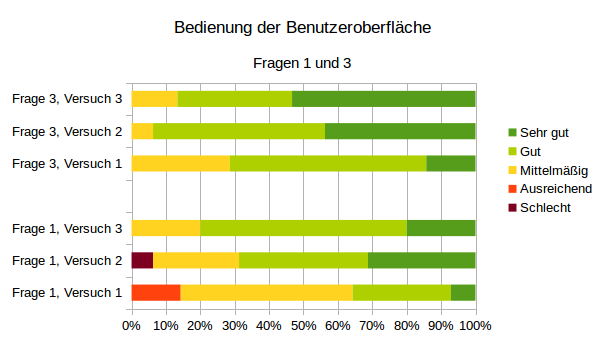
\includegraphics[width=0.95\textwidth]{./media/images/gui/trials/gui-f1-3.png}
\caption{Ergebnisse der Fragen 1 und 3}
\end{figure}

Hier ist besonders nach dem ersten Versuch ein deutlicher Fortschritt zu erkennen. Da bei dem Test mit der 2AHELS vor Allem am Anfang einige Probleme aufgetreten sind, haben wir uns nachher intensiver auf das Ausbessern dieser Fehler und das Verbessern der Stabilität von C Compact konzentriert.

Wir haben durch den ersten Versuch auch viele neue Ansichten und Ideen erhalten und konnten die Bedienbarkeit so sehr gut verbessern. Zum Beispiel war ein wichtiges Anliegen der ersten Versuchsgruppe eine bessere Fehleranzeige. Daraufhin führten wir in Version Alpha 1.2 anschauliche Fehlerbeschreibungen ein (siehe Kapitel \ref{sec:deb-error}).

Die letzte Versuchsgruppe hat gezeigt, dass die Benutzeroberfläche von C Compact sehr weit fortgeschritten ist. Immerhin haben 4 von 5 SchülerInnen angegeben, dass die Benutzeroberfläche \glqq{}gut\grqq{} oder \glqq{}sehr gut\grqq{} bewertet (Frage 1). Mehr als die Hälfte dieser Versuchsgruppe hat die C Compact als \glqq{}sehr intuitiv zu bedienen\grqq{} bewertet (Frage 3).

\subsubsection*{Ergebnisse: Fragen 4 und 5}

\emph{Frage 4: Wie anschaulich ist die Darstellung der Programmabläufe?\\
Frage 5: Wie verständlich werden die Variablen während des Programmablaufes dargestellt?}

\begin{figure}[h!]
\centering
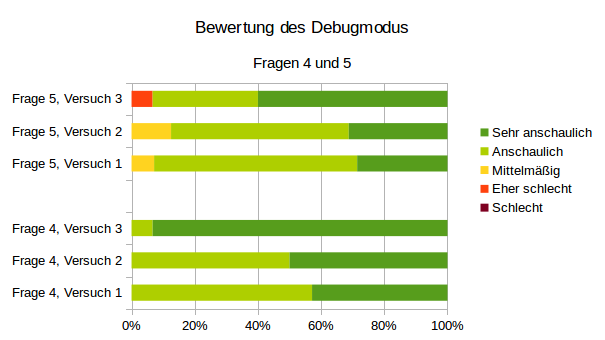
\includegraphics[width=0.95\textwidth]{./media/images/gui/trials/gui-f4-5.png}
\caption{Ergebnisse der Fragen 4 und 5}
\end{figure}

Der Debugger von C Compact wurde von Beginn an sehr positiv bewertet. Schon die erste Versuchsgruppe gab uns --- auch während der Übungsphase --- sehr positive Rückmeldungen. Eines der zentralen Konzepte von C Compact ist also erfolgreich aufgegangen.

Dass die Antworten der dritten Versuchsgruppe deutlich besser ausgefallen sind liegt einerseits daran, dass wir bis zur Version Alpha 1.4.2 einige Verbesserungen und zusätzliche Features zum Debugger hinzufügten. Andererseits vermuten wir, dass die SchülerInnen auch durch die eigene Einführungsübung (siehe Kapitel \ref{sec:sci-trials-gui-sched}) für den Debugger ein besseres Verständnis für dieses Tool entwickeln konnten. Ein wichtiger Aspekt für die Verwendung von C Compact im Unterricht ist also trotz der intuitiven Bedienbarkeit eine anschauliche Einführung.

\subsubsection*{Ergebnisse: Fragen 2 und 6}

\emph{Frage 2: Hast du Hilfe bei der Bedienung des Programms benötigt?\\
Frage 6: Häufigkeit von Bugs}

\begin{figure}[h!]
\centering
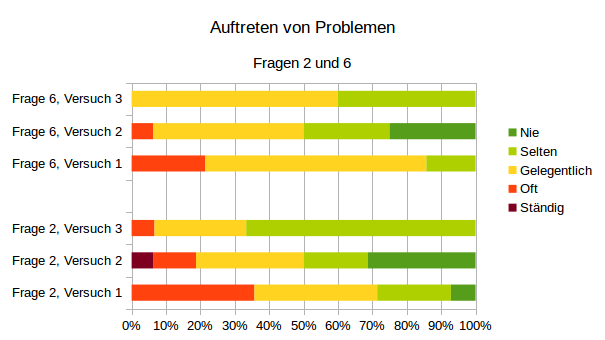
\includegraphics[width=0.95\textwidth]{./media/images/gui/trials/gui-f2-6.png}
\caption{Ergebnisse der Fragen 2 und 6}
\end{figure}

Obwohl besonders beim ersten Versuch einige Fehler aufgetreten sind, zeigte sich diese Versuchsgruppe sehr flexibel im Umgang mit Schwierigkeiten und in der Bedienung einer neuen Entwicklungsumgebung.

Nachdem wir viele Fehler notieren konnten, konzentrierten wir uns für die Version Alpha 1.2 vor Allem auf die Beseitigung von kleinen Abstürzen und Problemen. Im zweiten Versuch stürzte C Compact kein einziges mal ab. Größere Fehler zeigten sich nur vereinzelt. Dementsprechend fielen auch die Bewertungen positiver aus.

In der Version Alpha 1.4.2, die für den dritten Versuch verwendet wurde, gab es leider einen Bug, den wir durch eine Modifikation einige Tage zuvor verursachten und nicht bemerkten: Bei Fehlermeldungen wurde die falsche Zeile angezeigt. Dadurch hatten einige Schülerinnen und Schüler Probleme, die Fehler in ihrem Quelltext zu finden. Die Antworten auf Frage 6 sind dadurch wieder etwas negativer ausgefallen.

Einige Schülerinnen und Schüler gaben in Frage 2 an, hin und wieder Hilfe benötigt zu haben. Allerdings konnten zwei Drittel der Schüler laut eigenen Angaben fast selbstständig arbeiten und mussten nur selten Hilfe in Anspruch nehmen. Das lässt vor Allem auf eine gut durchdachte Aufgabenstellung und gute Erklärungen der benötigten Theorie und der Entwicklungsumgebung schließen.

\subsubsection*{Ergebnisse: Fragen 9 und 10}

\emph{Frage 9: Würde dir diese Entwicklungsumgebung im Unterricht helfen?\\
Frage 10: Würde dir diese Entwicklungsumgebung beim selbstständigen Lernen helfen?}

\begin{figure}[h!]
\centering
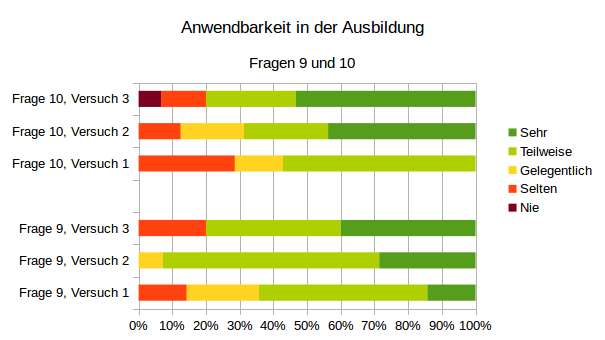
\includegraphics[width=0.95\textwidth]{./media/images/gui/trials/gui-f9-10.png}
\caption{Ergebnisse der Fragen 9 und 10}
\end{figure}

Mit dem Fortschritt von C Compact konnten sich auch immer mehr Schüler vorstellen, C Compact im Unterricht oder zum Üben zu verwenden. Wir erhielten immer wieder --- auch von den Lehrern der Versuchsgruppe --- positive Rückmeldungen. Im Prinzip zeigen diese Antworten, ob das Gesamtkonzept aufgegangen ist.

Wir vermuten, dass die schlechteren Bewertungen bei diesen Fragen von Schülern stammen, die sehr gute Programmierer sind und die mit einer professionellen Entwicklungsumgebung mehr anfangen können. Beispielsweise waren in der dritten Versuchsgruppe drei sehr gute Programmierer und bei den Fragen 9 und 10 in dieser Gruppe jeweils genau 3 schlechtere Bewertungen. Allerdings können wir in keinem der Fälle feststellen, ob diese Bewertungen tatsächlich von guten Programmierern kommen, da die Fragebögen anonym ausgewertet wurden.

\subsubsection*{Auswertung der Freitextfragen}

\emph{Frage 7: Welcher Bereich muss am dringendsten verbessert werden?\\
Frage 8: Was würdest du als nächstes hinzufügen?}

Die Antworten auf diese Fragen zeigten oft sehr gut die aktuellen Defizite von C Compact und brachten uns auch auf neue Ideen. Großteils waren die Antworten für beide Fragen sehr ähnlich.

Beim ersten und dritten Versuch zeigte sich das höhere Verbesserdungspotential auch dadurch, dass viele Schüler ähnliche Antworten gaben. Beim ersten Versuch 
gaben immerhin 9 Schüler an, dass als nächstes die Fehlermeldungen verbessert werden sollten (was wir dann auch taten) und 8 Schüler wünschten sich \textbf{for}-Schleifen als nächstes Feature. Beim dritten Versuch waren die wichtigsten Anliegen der Schüler einen Verbesserung der Fehlerkennzeichnung und -anzeige (die in der Version Alpha 1.4.2 nicht korrekt funktionierte). Die zweite Versuchsgruppe listete hingegen sehr unterschiedliche Ideen auf, was darauf hindeutet, dass keine signifikanten Probleme aufgetreten sind.
%TODO Anhang: Versuchsauswertungen.